\documentclass{article}
\usepackage[utf8]{inputenc}
\usepackage{tikz}
\usepackage{standalone}
\usepackage{amsmath}
\usepackage{amsfonts}
\usepackage[a4paper, total={6in, 9in}]{geometry}
\usetikzlibrary{shapes.geometric}


\newcommand{\bA}{\mathbf{A}}
\newcommand{\bB}{\mathbf{B}}
\newcommand{\bb}{\mathbf{b}}
\newcommand{\E}{\mathbb{E}}
\newcommand{\Norm}{\mathcal{N}}
\newcommand{\Loss}{\mathcal{L}}
\newcommand{\R}{\mathbb{R}}
\newcommand{\bt}{\mathbf{t}}
\newcommand{\bU}{\mathbb{U}}
\newcommand{\bu}{\mathbf{u}}
\newcommand{\bw}{\mathbf{w}}
\newcommand{\bX}{\mathbf{X}}
\newcommand{\bx}{\mathbf{x}}
\newcommand{\by}{\mathbf{y}}
\newcommand{\bZ}{\mathbf{Z}}
\newcommand{\bz}{\mathbf{z}}

\newcommand{\parfrac}[2]{\frac{\partial #1}{\partial#2}}

\title{Causal Effect Inference using Normalising Flows - background research}
\author{Micha de Groot}
\date

\begin{document}
\maketitle


%%%%%%%%%%%%%%%%%%%%%%%%%%%%%%%%%%%%%%%%%%%%%%%%%%%%%%%%%%%%%%%%%%%%%%
\section{Background research}

\subsection{causal inference, interventions, do-calculus and counterfactual reasoning}
The dominant research in artificial intelligence is all data-driven and broadly speaking looking for patterns in said data. The patters that most common AI models uncover are correlations between certain features in the data. In may problems this is a powerful tool that can perform a abundance of tasks, such as classification of images, translation of text or even the generation of new music. However, there is an inherent limit to models that can only uncover correlations: they can't find causal relation. Every class in statistics starts with the phrase: "Correlation is not causation." This mantra tells us that we should never interpret a correlation between a variable $A$ and variable $B$ as $A$ causes $B$. This is very much true, but sometimes we do like to know: does $A$ cause $B$? To answer such questions we need causal inference. 

In the causal inference framework, devised largely by Judea Pearl\cite{pearl1995causal} \cite{pearl2009causal}, we go beyond correlations by modelling the direction of cause and effect as well. This is done with Directed Acyclic Graphs (DAG); an example is given in Figure \ref{fig:graph_correlations_A_B}. Combined with structural equations for each edge in the graph, these form a Structural Causal Model. The parameters of these structural equations are similar to correlation coefficients except that the functions in which they are used have a clear direction. The estimation of such functions is what's called causal inference. 

\begin{figure}
    \centering
    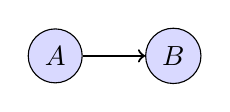
\begin{tikzpicture}
        \node[draw=black, circle, fill=blue!15!white] (a) at (0, 0) {$A$};
        \node[draw=black, circle, fill=blue!15!white] (b)at (1.5, 0) {$B$};
        \draw[->, thick] (a) -- (b);
    \end{tikzpicture}
    \qquad
    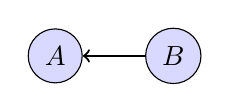
\begin{tikzpicture}
        \node[draw=black, circle, fill=blue!15!white] (a) at (0, 0) {$A$};
        \node[draw=black, circle, fill=blue!15!white] (b)at (1.5, 0) {$B$};
        \draw[->, thick] (b) -- (a);
    \end{tikzpicture}
    \qquad
    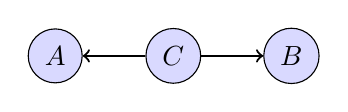
\begin{tikzpicture}
        \node[draw=black, circle, fill=blue!15!white] (a) at (0, 0) {$A$};
        \node[draw=black, circle, fill=blue!15!white] (b) at (3, 0) {$B$};
        \node[draw=black, circle, fill=blue!15!white] (c) at (1.5, 0) {$C$};
        \draw[->, thick] (c) -- (b);
        \draw[->, thick] (c) -- (a);
    \end{tikzpicture}
    \caption{Three possible DAGs for when $A$ and $B$ are correlated. On the left hand side $A$ causes $B$, in the middle $B$ causes $A$ and on the right hand side both $A$ and $B$ are caused by a third variable $C$.}
    \label{fig:graph_correlations_A_B}
\end{figure}

The reason we want to know the structure of these graphs and their corresponding functions is to answer causal questions. Although some cause and effect relations might seem deterministic, they are usually framed in a statistical fashion. This makes it possible to relate it to statistics and correlations, and in some cases even rephrase a causal question as a mere statistical one. The most important component in that regard is the \textit{do}-operator, see Equation \ref{equation:do_operation}. This equation tells us the probability of $A$ if we were to \textit{set} $B$ to a specific value; This is the causal effect from $B$ on $A$ in a probabilistic framing. The $pa_{B}$ is this equation indicates the set of all parents of $B$ in the causal graph, and if they are also parents of $A$ they are called confounders of $A$ and $B$. This immediately shows that we have to have knowledge of the causal graph to quantify a causal effect. For clarity  Equation \ref{equation:do_operation} also shows the conditional probability of $A$ given $B$ if we were to factor out the other parents of $A$. These two equations reduce to the same in certain cases, such as when $A$ has no parents, or when $B$ is the only parent of $A$. 
%Convince yourself that this is the case by looking back at Figure \ref{fig:graph_correlations_A_B}.

\begin{align}\label{equation:do_operation}
    p(A | do(B)) &= \int_{pa_B} p(A | B, pa_{B}) p(pa_{B}) \text{d} pa_B\\
    p(A | B) &= \int_{pa_B} p(A | B, pa_{B}) p(pa_{B}|B) \text{d} pa_B
\end{align}

Now the question arises: why is causal inference then perceived to be such a difficult problem if we can just slightly adjust an existing equation for computing conditional probabilities? This is because we either don't know the structure of the graph at all or if we can't observe certain confounders in the graph, called \textit{latent} confounders. If we don't know the graph we have to resort to causal discovery, which is beyond the scope of this research. If we do know the structure of the graph, or have strong indications to assume a certain structure, we can resort to methods to estimate the structural equations, even if not all variables are observed. The rest of this section will cover the existing work on causal inference in the case where there is a latent confounder.


% After that we will at some point talk about do-calculus and how you can measure a causal effect if you know the graph. Backdoor adjustment. Something about assuming a graph structure.

% Existing work on causal inference that doesn't use deep learning




\subsubsection*{Distinguishing cause from effect using observational data: methods and benchmarks}
--Book (chapter)\cite{mooij2016distinguishing}, quite long, will look for useful info--

Causal discovery in the bivariate case has been mostly based on the difference in complexity of the factorisation of the joint distribution $p(X,Y)$. If $p(X)p(Y|X)$ consists of two simpler distributions than $p(Y)p(X|Y)$ then it is likely that $X$ is a cause of $Y$ instead of the other way around. The chapter discusses several extensive benchmarks for these types of tests.

Another definition for "$X$ is a cause of $Y$" is that $p(Y|do(X=x)) \neq p(Y|do(X=x'))$




\begin{figure}
    \centering
    \includestandalone{Figures/causal_graph_one_proxy_one_confounder}
    \caption{Causal graph with one proxy variable. $\bt$ is the variable we intervene on; $\by$ is the outcome; $\bZ$ is the latent confounder; and $\bX$ is the observed proxy variable.}
    \label{fig:causal_graph}
\end{figure}
\subsection{Deep learning and Generative modelling}

\subsubsection*{Autoencoding Variational Bayes}
The problem of finding the posterior distribution of the latent variable of data is a problem that has been approached with different methods. Variational Inference is one of such methods, which has become very popular through the Variational Autoencoder(VAE) \cite{kingma2013auto}. The VAE is a framework that uses the principle of a variational distribution to approximate the posterior distribution. Because of the positioning of the VAE within the deep learning it was able to distinguish itself from other variational inference methods. 

The loss that a VAE optimises is called the Evidence Lower Bound (ELBO) or negative free energy. The name comes from the  fact that it is lower bound for the log likelihood $\log p_\theta(\bx)$, see Equation \ref{equation:negative_free_energy}. By using neural networks to parameterise the variational distribution and the likelihood, and the reparameterisation trick, it is possible to learn the variational distribution and the data likelihood, the two parts of the ELBO, through gradient descent methods.

\begin{equation}\label{equation:negative_free_energy}
    \begin{split}
    \log p_\theta(\bx) &= \log \int p_\theta(\bx | \bz) p(\bz) d\bz\\
    &= \log \int \frac{q_\phi(\bz|\bx)}{q_\phi(\bz|\bx)} p_\theta(\bx | \bz) p(\bz) d\bz\\
    &\geq -\mathbb{D}_{KL}[q_\phi(\bz|\bx) || p(\bz)] + \mathbb{E}_q[\log p_\theta(\bx|\bz)] = -\mathcal{F}(\bx)
    \end{split}    
\end{equation}
    

Although the VAE has been used successfully for variational inference, it does have its limits. A requirement for a VAE is that the variational distribution is a parameterised distribution that is chosen beforehand, usually a Gaussian with diagonal covariance. This of course limits the model in capturing more complex posterior distributions. Another disadvantage is that the likelihood tends to converge to a per-feature mean. This means that in datasets where individual features are either multimodal or are far from the mean, given a specific value of the latent value, the likelihood is fitted poorly on the data. This is apparent in image-based datasets. The images sampled from the model tend to be very blurry and lack sharp edges.

\subsubsection*{Variational Inference with Normalising Flows}
A normalising flows is a type of model that is capable of variational inference. Is is able to learn flexible, arbitrarily complex and scalable approximate posterior distributions. The main advantage it has over the VAE is that the approximation of the posterior is not limited to parameterised distributions. The idea is to start with a simple initial density that is parameterised, and transforming that into an arbitrary complex distribution by applying a series of invertible transformations. The final probability density is defined by applying the change of variable formula to the density of the original simple distribution, as shown in equation \ref{equation:change_of_variable}. The only requirement of the invertible mapping is that its Jacobian has to be efficiently computed, as it has to be evaluated many times, both during training and testing.

\begin{align}\label{equation:change_of_variable}
    \bz_K &= f_K \circ ... \circ f_1 (\bz_0)\\
    p(\bz_K) &= p(\bz_0) \prod\limits_{k=1}^K \left|\det \parfrac{f_k}{\bz_{k-1}} \right|^{-1}\\
    \log p(\bz_K) &= \log p(\bz_0) - \sum\limits_{k=1}^K \log \left|\det \parfrac{f_k}{\bz_{k-1}} \right|
\end{align}

\noindent
This can be applied by augmenting the VAE by taking the original, relatively simple, variational distribution and passing that through a series of such function, thereby reaching the more complex approximation of the posterior. The ELBO then has to be extended by substituting a part of it with the change of variable equation stated above. This is show in equation \ref{equation:negative_free_energy_with_flow}. Note here that this yields us an objective very similar to the original ELBO with just the log determinant Jacobian added to it.

\begin{equation}\label{equation:negative_free_energy_with_flow}
    \begin{split}
    -\mathcal{F}(\bx) &= -D_{KL}[q_\phi(\bz|\bx) || p(\bz)] + \E_{q_\phi(\bz|\bx)}[\ln p_\theta(\bx|\bz)]\\
    &= \E_{q_\phi(\bz|\bx)}[-\ln q_\phi(\bz|\bx) + \ln p(\bz) + \ln p_\theta(\bx|\bz)]\\
    &= \E_{q_0(z_0)}[-\ln q_0(\bz_K) + \ln p(\bz) + \ln p_\theta(\bx|\bz_K)]\\
    &= \E_{q_0(z_0)}[-\ln q_0(\bz_0) + \sum\limits^K_{k=1}\ln \left|\text{det} \parfrac{f_k}{\bz_{k-1}} \right| + \ln p(\bz) + \ln p_\theta(\bx|\bz_K)]\\
    &= -D_{KL}[q_0(\bz_0|\bx) || p(\bz)]+   \E_{q_0(z_0)}[\sum\limits^K_{k=1}\ln \left|\text{det} \parfrac{f_k}{\bz_{k-1}} \right| + \ln p_\theta(\bx|\bz_K)]\\
    \end{split}
\end{equation}

\noindent
Rezende and Mohamed also propose two possible functions that fulfil the requirement of having a tractable log determinant Jacobian, called the Planar Flow and Radial Flow. Both these functions consist of a residual connection to which a simple transformation to the input is added. Even though both of these flow types apply a small change per function, they can reach a complex transformation by stacking enough of them.

%The negative free energy function $\mathcal{F}$ is also known as the Evidence Lower Bound(ELBO). The novelty of normalising flows lies in how the approximate posterior $q_\phi(\bz|\bx)$ is defined.  


\subsubsection*{Density estimation using Real-NVP}
The Normalising Flows paradigm has given rise to several other models, one of which is the Real-NVP \cite{dinh2016density}. The Real-NVP also work by chaining a series of invertible functions that have a tractable log determinant Jacobian. Dinh et al. have achieved this by designing so-called coupling layers. These coupling layers each apply a translation and scaling to a part of the current input. The other half is copied, see Figure \ref{fig:real_nvp_graph}. By changing which part is copied and which is altered every coupling layer you can reach complex transformations to your whole vector. The scaling and translation of one half of the vector are determined by neural networks that each take the other half of the vector as input. Fortunately the log determinant Jacobian of the coupling layer does not require the determinant of the neural networks, meaning those networks can be arbitrarily complex.

\begin{figure}
    \centering
    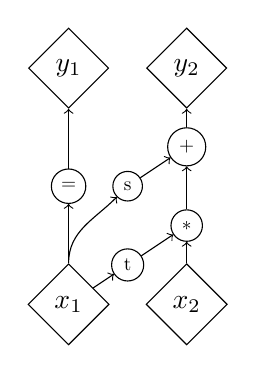
\begin{tikzpicture}
        \node[draw, diamond] (y1) at (0,0) {$y_1$};
        \node[draw, diamond] (y2) at (1.5,0) {$y_2$};
        \node[draw, diamond] (x1) at (0,-3) {$x_1$};
        \node[draw, diamond] (x2) at (1.5, -3) {$x_2$};
        \node[draw, circle, scale=0.7] (+) at (1.5, -1) {$+$};
        \node[draw, circle, scale=0.7] (=) at (0, -1.5) {$=$};
        \node[draw, circle, scale=0.7] (*) at (1.5, -2) {$*$};
        \node[draw, circle, scale=0.7] (s) at (0.75, -1.5) {s};
        \node[draw, circle, scale=0.7] (t) at (0.75, -2.5) {t};
        
        \draw[->] (x1) -- (=);
        \draw[->] (=) -- (y1);
        \draw[->] (x1) edge[out=90, in=225] (s);
        \draw[->] (x1) -- (t);
        \draw[->] (s) -- (+);
        \draw[->] (t) -- (*);
        \draw[->] (x2) -- (*);
        \draw[->] (*) -- (+);
        \draw[->] (+) -- (y2);
    \end{tikzpicture}
    \qquad
    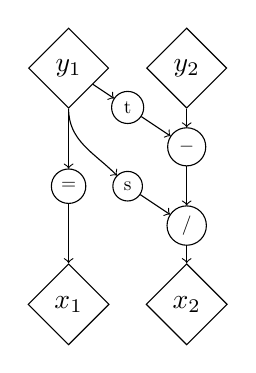
\begin{tikzpicture}
        \node[draw, diamond] (y1) at (0,0) {$y_1$};
        \node[draw, diamond] (y2) at (1.5,0) {$y_2$};
        \node[draw, diamond] (x1) at (0,-3) {$x_1$};
        \node[draw, diamond] (x2) at (1.5, -3) {$x_2$};
        \node[draw, circle, scale=0.7] (-) at (1.5, -1) {$-$};
        \node[draw, circle, scale=0.7] (=) at (0, -1.5) {$=$};
        \node[draw, circle, scale=0.7] (/) at (1.5, -2) {$/$};
        \node[draw, circle, scale=0.7] (s) at (0.75, -1.5) {s};
        \node[draw, circle, scale=0.7] (t) at (0.75, -0.5) {t};
        
        \draw[->] (y1) -- (=);
        \draw[->] (=) -- (x1);
        \draw[->] (y1) edge[out=270, in=135] (s);
        \draw[->] (y1) -- (t);
        \draw[->] (s) -- (/);
        \draw[->] (t) -- (-);
        \draw[->] (y2) -- (-);
        \draw[->] (-) -- (/);
        \draw[->] (/) -- (x2);
    \end{tikzpicture}
    \caption{Coupling layer of the Real NVP and its inverse}
    \label{fig:real_nvp_graph}
\end{figure}

\subsubsection*{Analyzing Inverse Problems with Invertible Neural Networks}
The invertbility of flow-based models makes them suitable for recovering posterior information of complex physical systems. This has been proposed by Ardizzone et al. \cite{ardizzone2018analyzing} in the form of Invertible Neural Networks. Given some process $\bx \rightarrow \by$ with observed $\by$ and unobserved $\bx$ oe would like to know how to recover $\bx$ for a ceartain $\by$. This is done by using an approach based on the Real-NVP\cite{dinh2016density} model. Since the forward process has inherent information loss, a latent variable $\bz$ is introduced that captures the information in $\bx$ that is not contained in $\by$, turning the process into $f(\bx) = [\by, \bz]$  and $\bx = f^{-1}(\by, \bz) = g(\by, \bz)$. Because of the nature of Normalising-Flow models, $g(\by, \bz)$ does not have to be modelled separately. The density $p(\bz)$ is shaped as a Gaussian. 

This differs from the causal graph in Figure \ref{fig:causal_graph} because both $\bx$ and $\bz$ are unobserved. Though the INN approach might still be useful if we were to recover $\bZ$ from a given $\bX$. I think this would be an approximation for $p(\bZ | \bX)$, which could then be used to approximate equation \ref{equation:intervention}. 


\subsubsection*{Sylvester Normalising Flows for Variational Inference}
Another flow-based model is the Sylvester Normalising Flow\cite{berg2018sylvester}. This is a direct adaptation of the planar flow designed by Rezende and Mohamed. The planar flow function consist of a residual connection and a linear layer with a bottleneck of one dimension (and a non-linearity), see equation \ref{equation:planar_flow_sylvester_flow}. The reason for that is to have a closed form solution of the log determinant Jacobian. Van den Berg et al. came up with a version that does not require a bottleneck of one dimension, allowing the mappings to learn far more transformations.

\begin{align}\label{equation:planar_flow_sylvester_flow}
    f_{planar}(\bz) &= \bz + \bu h(\bw^T\bz + b)\\
    f_{sylvester}(\bz) &= \bz + \bA h(\bB\bz + \bb)
\end{align}

By making use of Sylvester's determinant identity and a QR-factorisation of matrices $\bA$ and $\bB$ in equation \ref{equation:planar_flow_sylvester_flow}, the transformation can be rewritten in such a way that it has a tractable Jacobian. The resulting matrices $Q$ and $R$ of the QR-factorisation do have to be kept orthogonal and triangular respectively. The paper by van den Berg et al. proposes several methods to do this during training.

\subsubsection*{Generative Adversarial Networks}
A Generative Adversarial Network (GAN) is another type of generative model\cite{goodfellow2014generative}. It differs from the model described above in several aspects. Firstly is doesn't model the posterior of the data in any way, it only models the prior and the likelihood. This is of course a downside of the model, but what it brings to the table is this: it uses adversarial learning to train the generator model. Instead of learning a mean squared error of each individual feature it concurrently trains another model, the discriminator model, that must label the generated image as either a real image from the dataset or a generated one. This classification error is the only thing that is backpropagated, both through the discriminator and the generator. The result of this is, in the case of an image dataset, a model that is capable of generating far sharper images than a VAE could. 

Because there is no posterior, a GAN can only generate completely random images. To allow some selection in what the model would generate, the conditional GAN was created \cite{mirza2014conditional}. A conditional GAN extend the GAN by conditioning the input of the generator not only on a random sample of the prior, but also on a conditional vector that represents a visual feature such as the person in the image having a moustache.  



%%%%%%%%%%%%%%%%%%%%%%%%%%%%%%%%%%%%%%%%%%%%%%%%%%%%%%%%%%%%%%%%%%%%%%
\section{Related work: Intersection of generative modelling and causal inference}
In the last few years there have been several papers that have tried to use the power of generative modelling in causal inference to try to learn causal relations from observational studies when a lot of data is available. There also has been research that tried to approach typical deep learning problems from a causal viewpoint in cases where it was beneficial to explicitly take causal relations in the data into account.

\subsubsection*{Causal Effect Inference with Deep Latent-Variable models}
The paper by Louizos et al.\cite{louizos2017causal} serves as a good starting point for research into the use of generative modelling in causal inference. It explores the possibility of measuring the direct effect of one observed variable on another given that there is a shared unobserved confounder by using a proxy variable that has the same confounder. This causal graph is shown in Figure \ref{fig:causal_graph}. Their contribution is doing this task by using Variational Autoencoders\cite{kingma2013auto} to recover the Individual Treatment Effect(ITE):
\begin{equation}\label{equation:ITE}
    ITE(x) := \mathbb{E}[\by | \bX = x, do(\bt = 1)] - \mathbb{E}[\by | \bX = x, do(\bt=0)]
\end{equation}

\noindent
The paper states that $\bt$ does not have to be binary for their approach to work but it is assumed for simplicity and compatibility with prior benchmarks. First the joint distribution $p(\bZ, \bX, \by, \bt)$ is approximated with a VAE that consists of several neural networks. With that $p(\by | \bX, do(\bt=1))$ can be identified:

\begin{equation}\label{equation:intervention}
    \begin{split}
    p(\by | \bX, do(\bt=1)) &= \int_\bZ p(\by | \bX, do(\bt=1, \bZ)) p(\bZ | \bX, do(\bt = 1)) d\bZ \\
                            &= \int_\bZ p(\by | \bX, \bt = 1, \bZ) p(\bZ | \bX) d\bZ
    \end{split}
\end{equation}

\noindent
The inference network captures $q(\by | \bt , \bX), q(\bZ | \bt, \by, \bX), q(\bZ| \bt, \by, \bX)$ and the generative network captures $p(\bX | \bZ), p(\bt | \bZ), p(\by | \bt, \bZ)$. These are then used to compute a sample average for the ITE.

%The problem with trying to translate this to Normalising-Flow model is that an NF model cannot simply model conditional distributions. For this we would require a way to model arbitrary Bayesian networks with NF. 


\subsubsection*{CausalGAN: Learning Causal Implicit Generative Models with Adversarial Training}
The CausalGAN\cite{kocaoglu2017causalgan}. converts the conditional GAN to a causal GAN, which allows the model to intervene on features instead of conditioning on them. Examples are features such as the person in the image having a moustache. With intervening on that feature instead of conditioning the model can for example generate images of women with moustaches.

As this model is GAN-based

\subsubsection*{A Meta-Transfer Objective for Learning to Disentangle Causal Mechanisms}
Disentanglement with causality \cite{Bengio2020A}

\subsubsection*{Causal Confusion in Imitation Learning}
Within imitation learning\cite{torabi2019recent} there is a problem, called causal confusion by de Haan et al.\cite{de2019causal}. This problem arises when there is a feature that is observed by the learner that is highly correlated with the action that the expert takes. However, it is not an indicator that the action should be taken, rather it is an effect that is caused by taking the action. This causes problems for the learner when there is a distributional shift from the training data to the test data, which is always the case in imitation learning. De Haan et al. try to solve this problem by simultaneously learning the causal graph between actions and observations, and which actions lead to a better performance. They show that the learned graph does indeed correspond to the factor that would cause the expert to take a certain action and that the learning agent performs better or equal on benchmarks such as Atari games than the state-of-the-art. 

% We don't explicitly look for the graph by masking latent variables in the decoding, but we do provide a label on what intervention was applied. That is somewhat similar to their expert telling which action it took. We also won't do any actual RL. But Pim doesn't model a prediction from the result of the action, only which action is a 'good' action. Our model can potentially be used for more general queries. Also our interventions aren't discrete.

This research is similar to our approach in the sense that it must learn the effect from an intervention or action by observing visual data. Our approach doesn't involve an explicit learning of the causal connections between each latent variable and the interventions, but instead aims at learning the effect of more complex interventions than the set of discrete actions that is available in a typical reinforcement learning setting. This potentially leads to a model that can predict more complex effects from interventions on a video frame than what the intervention or action is that leads to the highest return.



\subsubsection*{Causal Correct Partial Models for Reinforcement Learning}
Causally correct RL: \cite{rezende2020causally}

\subsubsection*{Discovering causal signals in images}
Lopez et al. have investigated the possibility of learning causal signals from visual data \cite{lopez2017discovering}. Their idea was that the presence of certain objects must have been a cause for the presence of other objects in the image. For instance, the presence of a car in an image is a (stochastic) cause for the presence of wheels in the image. 

The paper does look at causal relations within image scenes, but it never models interventions. It only looks if neural net can find correlation between features that are part of objects that have causal relations. It is good to know that a model is capable of distinguishing such features, since we need it for our problem as well.

\subsubsection*{VideoFlow}
The idea of Normalising Flows has also been adapted for video generation, where the model takes a few frames as input and predict the next few frames. This model is called the VideoFlow\cite{kumar2019videoflow}. The basic principle behind the model is that it uses the idea of coupling layers from the Real-NVP to generate frames from the latent vector at that timestep and combines that with an autoregressive prior distribution of the latent vectors, to condition them on all earlier time steps. Because it is a Flow-based model the log-likelihood can be optimised directly and generate frames efficiently compared to a pure autoregressive model.

In a sense it goes beyond what we are trying to achieve because it can predict more than one frame in the future. Though it doesn't distinguish between the role objects and actors play in a scene. It might be a good idea to make use of their architecture for the generation of images/frames from a latent vector.



\bibliography{references.bib}
\bibliographystyle{abbrv}

\end{document}
